\documentclass[12pt]{article}
\usepackage[pdfborder=0 0 0]{hyperref}
\usepackage[utf8]{inputenc}
\usepackage {babel}
\usepackage{graphicx}
\usepackage{pdfpages}
\usepackage{attachfile}
\DeclareGraphicsExtensions{.pdf, .png, .jpg, .jpeg}
\graphicspath{{./graphics/}}
\title{
    Quality of Service - FFI \\
    IT2901 - Group 7  \\ 
    Preliminary Report \\
}
\author{
    Bremnes, Jan A. S. \\  
    Johanessen, Stig Tore \\
    Kirø, Magnus L.\\
    Nordmoen, Jørgen H.\\ 
    Støvneng, Ola Martin T.\\
    Tørresen, Håvard \\
}
\date{\today}

\begin{document}
\maketitle
\titlepage
\pagenumbering{arabic}
\newpage

\begin{abstract}\label{abstract}
This is the paper's abstract \ldots
\end{abstract}

\tableofcontents
\listoffigures
\listoftables
\newpage

\section{Project Introduction}\label{intoduction}
    This report is intended to guide you, through our work, decisions and results. This report will detail how we planned the project, how we designed the architecture and how we tested and evaluated the result. Hopefully by the end of this report you will understand how and why we made the decisions that we did, and additionally we hope you will enjoy or work in the same way that we have enjoyed working on it. We have intended for the results to be both verifiable and interesting for the right audience and we hope our customer will be pleased with it. If we have done this report right you will, by the end, be able to take an informed decision about how and why you should implement quality of service in networks were bandwidth is a scarce resources.

\section{Task Description and Requirements}\label{taskdescreq} 
    Our task is to provide a Quality of Service (QoS) layer to web services for use in military tactical networks. As these networks tend to have severely limited bandwidth, and our QoS-layer must therefore prioritise between different messages, of varying importance, that clients and services want to send. Our middleware will have to recognize the role of clients, and, together with the service they are trying to communicate with, decide the priority of the message.
    
    \subsection{Description}\label{taskdesc} 
    [Description of the task at hand.]
        
    Our assignment is to create a Java application which will function as a middleware layer between web services, and clients trying to use these services. The middleware needs to process SOAP messages, which is the communication protocol for most web services, in order to be able to do its task. On the client side, the middleware needs to process messages and understand SAML in order to deduce the role of the client. This role, together with information about the service the client is trying to communicate with, decides the overall quality of service the messages should receive. 

    Our middleware needs to be able to modify the TOS/Diffserv IP packet header in order for the tactical router to prioritize correctly. Currently NATO has just defined one class, BULK, which is to be used with web services, but this may change in the future and our middleware should handle this upcoming change gracefully.

    In addition to this, the middleware needs to be able to retrieve the available bandwidth in the network, which in the real system will be retrieved from the tactical routers. In our testing this information will come from a dummy layer, but how this information is obtained should also be very modular, so that the customer can change how the bandwidth information is obtained later.

    With all this information, the role of the client, the relationship between the client and the service, and the available bandwidth, our middleware layer should be able to prioritize messages. Our product should, as much as possible, use existing web standards, the customer outlined some of their choices and options we have for implementation, like SAML, XACML, WS-Security and WSO2 ESB. In addition to this, our middleware needs to work with GlassFish, as that is the application server the customer uses.
   
    \subsection{Requirements}\label{taskreq}
    \begin{itemize}
        \item Written in java
        \item High priority messages must arrive, even at the cost of dropping lower priority messages.
        \item Use standards where they can be used
            \subitem SAML
            \subitem Diffserv
            \subitem XACML
            \subitem WS-Security
        \item Test thoroughly
            \subitem Use NS3 for testing
        \item Extensive documentation
        \item Use metadata to determine priority
        \item GlassFish must be supported as the application server
        \item Must be able to set priority on network layer packets
            \subitem Currently there is only one priority class defined by NATO, the BULK class, but this will most likely change in the future, as such our middleware layer needs to be expandable enough to handle this change in the future.
        \item There are no requirements on resource usage, but we should try to keep it lightweight.
            \subitem The customer has only said that we can expect the product to be used on a standard laptop with full Java support
    \end{itemize}
    
\section{Project Management}\label{management} 
    In this section, we'll take look at how we organized the team, a brief risk assesment, and an evaluation of the work process 
    
    \subsection{Team Organization}\label{team} 
        [The team structure and roles.]
    
    We already know each other coming into the project so we’ve chosen a flat organisational structure, since all decisions within the team will more or less be made by all the members together either way. Relying on the entire group for decisions will both involve and invest everyone in the project and will work well with our already existing group dynamic.

    Since this is a research project, the customer will act more as an advisor than a customer, and will have more suggestions and advice than demands and requirements. We have been given a clear understanding of what the final product should be, and we have a list of requirements that should be met. Other than that, we are relatively free regarding how we go about solving the problem. Because of this, a methodology like Scrum won't work for us, as it requires us to be in close and frequent contact with the customer, presenting a prototype every other week and continue development based on the customers feedback and demands.

    The customer does not require any prototypes along the way, just a working prototype by the end of the project, so the deadlines we have set for the alpha and beta, are self-imposed.
    
    \subsection{Risk Assesment}\label{risk}
    
    \subsection{Process Evaluation}\label{processevaluation}
    
\section{Project Methodology}\label{methodology} 
    We did not follow any established development methodology, such as Scrum or XP, as this project required more planning and configuration of existing solutions, than actual coding. We therefore chose a mix of waterfall and agile methods, we discuss these decisions in the sections below. You will also find a list of the tools we chose to work with, and why we decided to use them. 

    \subsection{Project Organization}\label{projectorg}[How we organize the project]

    As the customer wanted all documentation written in English, we decided to use this for all written communication and documentation, in order to keep things consistent.

    We will work together from 10 to 16, Monday through Thursday every week, with allowed exceptions for lectures and such. Group members can also work in their free time to make up for missed collaboration hours or to just put in some extra work. This means more work than the course requires, but we decided that we want to do it this way so we can either take some time off now and then, or have more time for the exams in May.

    The customer has not given us many strict requirements, but instead they have suggested a few things that we could do. Given this freedom, we decided that we should improve on the base requirements by adding most of the things mentioned in this section.

    This is a project that requires quite a lot of planning before any programming can be done. This necessitates that we start the development according to a waterfall model in terms of the architecture planning as well as the requirements specification.
    
    As the project progresses we’ll be switching to a more agile development method, so as to allow for iterative development and facilitate for any necessary changes that may turn up as code is produced. Agile also allows for a far flatter organisational structure, which we believe will greatly help cooperation within the team.
    
    The way the course is structured in terms of deliveries of reports and documentation also creates a fairly natural implicit sprint period to work off of, and using an agile methodology will help in easily producing and maintaining said reports and documentation. In addition to the  reports and documentation, we will try to deliver two prototypes, an alfa and a beta version, to the customer before the final delivery in May.

    We will not be able to have face to face meetings with the customer, but we will have weekly online meetings with them instead, as well as e-mail communication as needed. Since we have seen what happens in projects where there is little to no communication, we decided, in agreement with the costumer, that we at least wanted to have weekly meetings in order  to keep a good dialog with the customer, and also give them the opportunity to take part in the development of the project. Since we have some challenges in the fact that the customer is in Oslo, we decided that the weekly meetings will be held over Skype.

    We  intend to do a test driven development in order to achieve high quality code. This will give us something to test while we are working, and it will also give us a great way to tell if some new piece of code gets in the way of previously written code. For this purpose we will use JUnit as the testing framework. We will also be doing periodical code reviews approximately every two weeks of development, synchronized with a code/feature freeze where we make sure everything works. As the customer wanted extensive testing of the middleware, we agreed to do testing on the network emulator NS3, as we have someone in the group already familiar with it. The advantage of using NS3 will be extensive testing, but also a great deal of empirical and verifiable data, which the customer also can use to evaluate the product.

    We will use Git and GitHub to handle our file repository, although Google Docs will be used for easy sharing and collaboration of schedules, meeting minutes, and reports. Even though the course set us up to use Subversion, we decided against this as Git gives us more options to develop code which will not greatly effect other parts of the codebase before we decide to integrate it. To this extent we have decided that as much as possible we should take advantage of Git’s built in support for ‘branches’. The argument for using Google Docs is that we have the possibility of editing a document together and easy sharing of documents. Delivered reports will be created with LaTeX, which we prefer over standard word processors.

    Each of us is free to choose his own IDE for programming. Because we are using Git, there should be no problem in using the IDE of our choice, and this gives us the added advantage that each person can use the tool which he is most comfortable with. We will stick to the standard Java Coding Conventions.

    \subsection{Tools}\label{tools} [The tools that we will use in the project.]
    
    Since we were so free to chose which tools we wanted to use we decided that this list should be quite lightweight. However the list compiled should be an indication of what is needed for the project. Some of the tools were chosen by us as is and other were demanded by needs of other components. All tools used can be  upgraded, downgraded or dropped during the course of this project. The final report will contain the official list as such this list is not in any way final. Our final report will also contain a list with supported tools tested with the final product.
    \begin{itemize}
        \item Git version 1.7.x
        \item Java version 1.6.x
        \item Free choice of IDE
        \item JUnit version 4.x
        \item NS3 unknown at present time
        \item WSO2 ESB 4.0.3
    \end{itemize}
    
\section{Prestudy}\label{prestudy} This project is one that requires quite a lot of prestudy before we can begin coding or even designing the architecture. Since the customer wanted us to implement existing technologies, such as Glassfish, WSO2, SAML etc. we need to spend some time researching those technologies to figure out what to use, and how to use it. The following sections will describe the overall architecture of how we, at this point in time, imagine our system will be like. 

    \subsection{Server side Architecture}\label{serversidearch} [The architecture of the server side module we are to create.] 
    
        The server side architecture consists of several components, the WSO2 ESB, the WSO2 Identity Server, the Tactical Router and the GlassFish server. All of these components are already available, so what we will have to make is mediators in the ESB.

        Before the client can request a web service it has to have an identification. To get an ID-token it has to contact the Identity Server using the ESB as a proxy (1). Then the client can request a web service from the ESB. Several things will then happen in the ESB. First the request message is sent to the SAML mediator (2), this mediator contacts the Identity Server to validate the clients ID-token (3). If the token is validated and the client is supposed to have access to the requested service the message is passed on to the GlassFish proxies (4), otherwise it is dropped. The ESB acting as a proxy will then send the request along to the requested service on the GlassFish server (5).
        
        \begin{figure}[htb]
            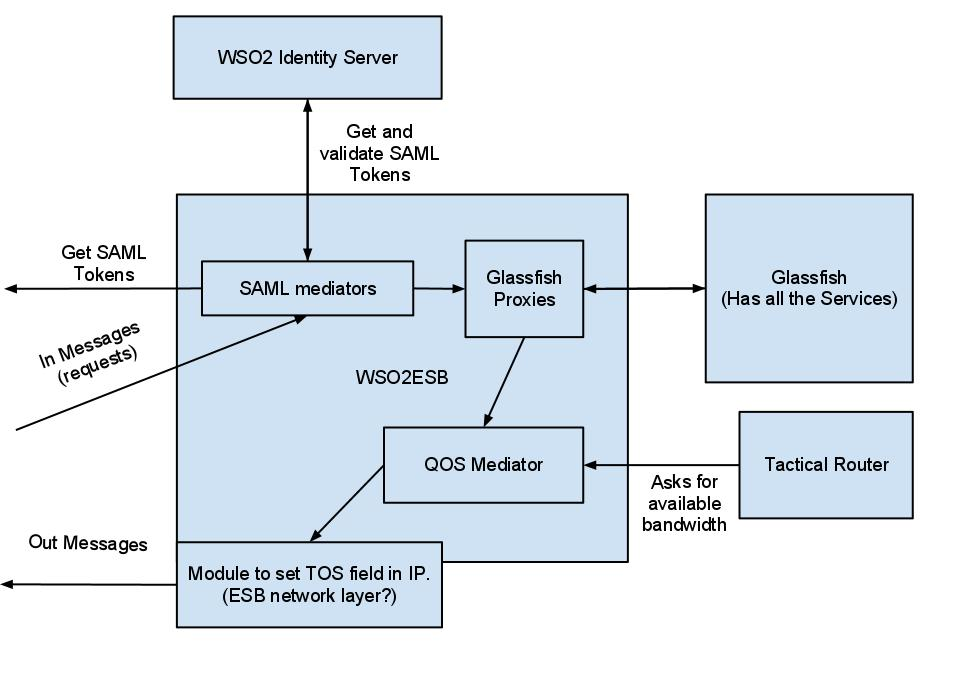
\includegraphics[scale=0.4]{serverside}
            \caption{The Server side Architecture}
            \label{fig:serverside}
        \end{figure}

        When the request is received at the service, it will probably start sending some data to the client. This is also done through the ESB. First the message is sent to the QoS mediator (6). This mediator will first look at the role, or identity, of the client and the service requested, and use this information to assign a priority to the connection. Then the Tactical Router is contacted for bandwidth information (7), which is used together with the priority to determine whether the message should be sent right away or held back until some higher priority message is finished sending.

        Either in the QoS mediator, in the ESB’s network layer, or after that, the Diffserv (ToS) field of the IP header will have to be set (8) before the message is sent to the client (9). This field is used by the routers in the network to prioritize packet sending. This step is quite important to the whole procedure as this is one of the few requirements the customer has given us, as such this step can not be dropped from the final product.

    \subsection{Client side Architecture}\label{clientsidearch} [The architecture of the client side module we are goint to create.] 
    
        The client-side architecture will be composed of altered (already existing) client software, the OpenSAML library as well as our client library implementation.
        
        \begin{figure}[htb]
            \centering
            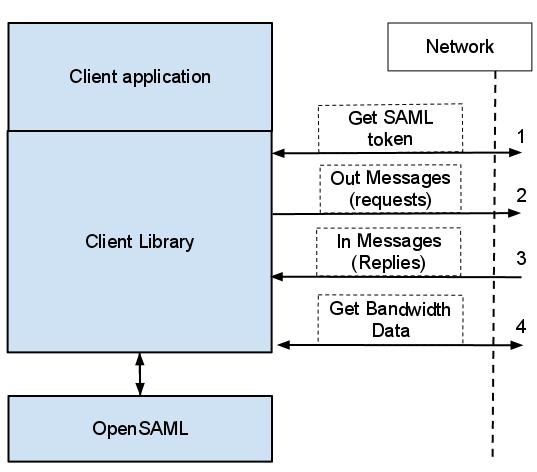
\includegraphics[scale=0.4]{clientside}
            \caption{The Client side Architecture}
            \label{fig:clientside}
        \end{figure}
 
        Before the client library can ask for the data the client needs to get a SAML authentication token from the identity server (1). The communication here will most likely be handled by our library, but the SAML packages will be created and analyzed by the OpenSAML library. 

        The client library then sends the request from the client to the server (2), appending the SAML token to the package as well as adding some metadata in the SOAP header related to the client role and setting the TOS field of the package to a default value.

        The reply from the server is examined by our client library for the metadata the server has embedded in the SOAP header, relevant metadata is stored for future communication and the package is passed to the client application (3).

        When new communication is initiated after this first connection is made the client should, if everything went as expected, have the necessary information to prioritize new messages. This means that the client can now take quite an informed decision about how it should prioritize messages, but in order to do this to the best of it’s abilities it also has to take into consideration available bandwidth (4).
    
           
    \subsection{Alternative solutions}\label{alternativesolutions} [Sollutions that we have, thought about but discarded.]
    
        Since this is only the preliminary report we have not yet decided on a final solution to the task at hand. But we have taken some decisions which will influence alternative solutions and will lock out some possible avenues of research.

        Since you can see an outline to the architecture in \ref{prestudy} we will instead use this section to outline some of the alternative architectures which we looked at, but rejected for the moment.

        The customer also gave us a paper(\cite{soa-qos-pdf}) which described a previous project they had worked on which tried to solve something quite similar to what we were tasked with. The paper described a system which were used in conjunction with Tactical routers(\ref{glossary}) to retrieve bandwidth information and to control sending of messages into this network. As the customer explained this work was not something we could directly copy as the project had not used a lot of web standards and had focused more on the tactical routers as opposed to web services. What we could take out of it however was how they throttled messages. The paper contained five methods which we could easily implement and use their result as an indication of what methods we should use to throttle or hold back messages.

        One architecture, which our customer suggested for the project, was to have a proxy in between nodes and creating a custom QoS layer which would sit in front of both the client and the services. This layer would then communicate with a SAML server for authentication, and would have to do all the message prioritization based on the same criteria as our architecture. There are several points about this architecture which would make it a good fit for us. Since the QoS layer would be identical on both client and server side it would mean less work, and more code that could be shared among components, but this freedom comes with some downsides. The first and most glaring problem encountered would be that services on the server would have to be altered to be able to communicate with this front end. Even though we were free to choose architecture ourselves, the client expressed a wish that we would not choose this model because the customer wants to use COTS(\ref{glossary}) services which would not be compatible with the new front end.

        Even though the above mentioned architecture is not the best fit for us we wanted to take some aspects of the architecture further. Since clients can easily be altered, the above mentioned solution is not applicable for server side, the solution could however be used for the clients. Having a proxy on the client side could be quite good, but because of the work involved and probable time constraints we chose not to go with this solution. On the server side however a front end is not the best solution for us. What we instead are looking into, is to use an ESB\ref{glossary} which would be configured together with the services and work as a proxy. Because many ESBs have integrated SAML processing we could easily take advantage of such facilities along with custom message processing, with which we would then extend the ESB to support our needs. The clients would have to point to the ESB, but this should both be trivial to do and the customer has expressed their agreement that this is satisfactory. We could eventually expand the functionality with service-discovery, which then would be a good solution to the problem.

        So far we have outlined major alternative architectures which could be alternatives to our project, but there are also alternatives within our proposed solution. One such alternative is not to use a premade ESB, but rather build one ourselves. This solution was thoroughly investigated, but was eventually turned down because of the massive amount of work that had to be done, the quality of an already made ESB is much higher than we could ever achieve during this project, and lastly, the opensource tools available to implement the functionality needed for SAML was not very well documented, and would take considerable time to get familiar with.

        On the client side we also have the choice of having either a HTTP proxy or writing our own custom library. Both have some advantages and disadvantages, a proxy would be better for integration with client programs, but creating this proxy or configuring and customizing an already existing solution is not trivial. On the same note, creating a library for use in client programs is easier, but this would mean that client programs would need to be altered to be usable with our middleware, which isn’t that desirable. We chose to go down the road of least resistance, as we see it currently we would have do quite a lot of research into proxies which could in the worst case scenario result in just wasted time as far as our product goes. A client library would from our perspective be easier as we would have more control, the overall design should be easier and we know that with this sort of library we can integrate OpenSAML which is a huge advantage.  
              
\section{Design}\label{design}
\section{Implementation}\label{implementation}
\section{Testing}\label{teting}
\section{Results}\label{results}
\section{Conclusion}\label{conclusion}
    \subsection{Future Work}\label{future}
\section{Project Evaluation}\label{evaluation}

\appendix
\section{Techical Glossary}\label{glossary}
    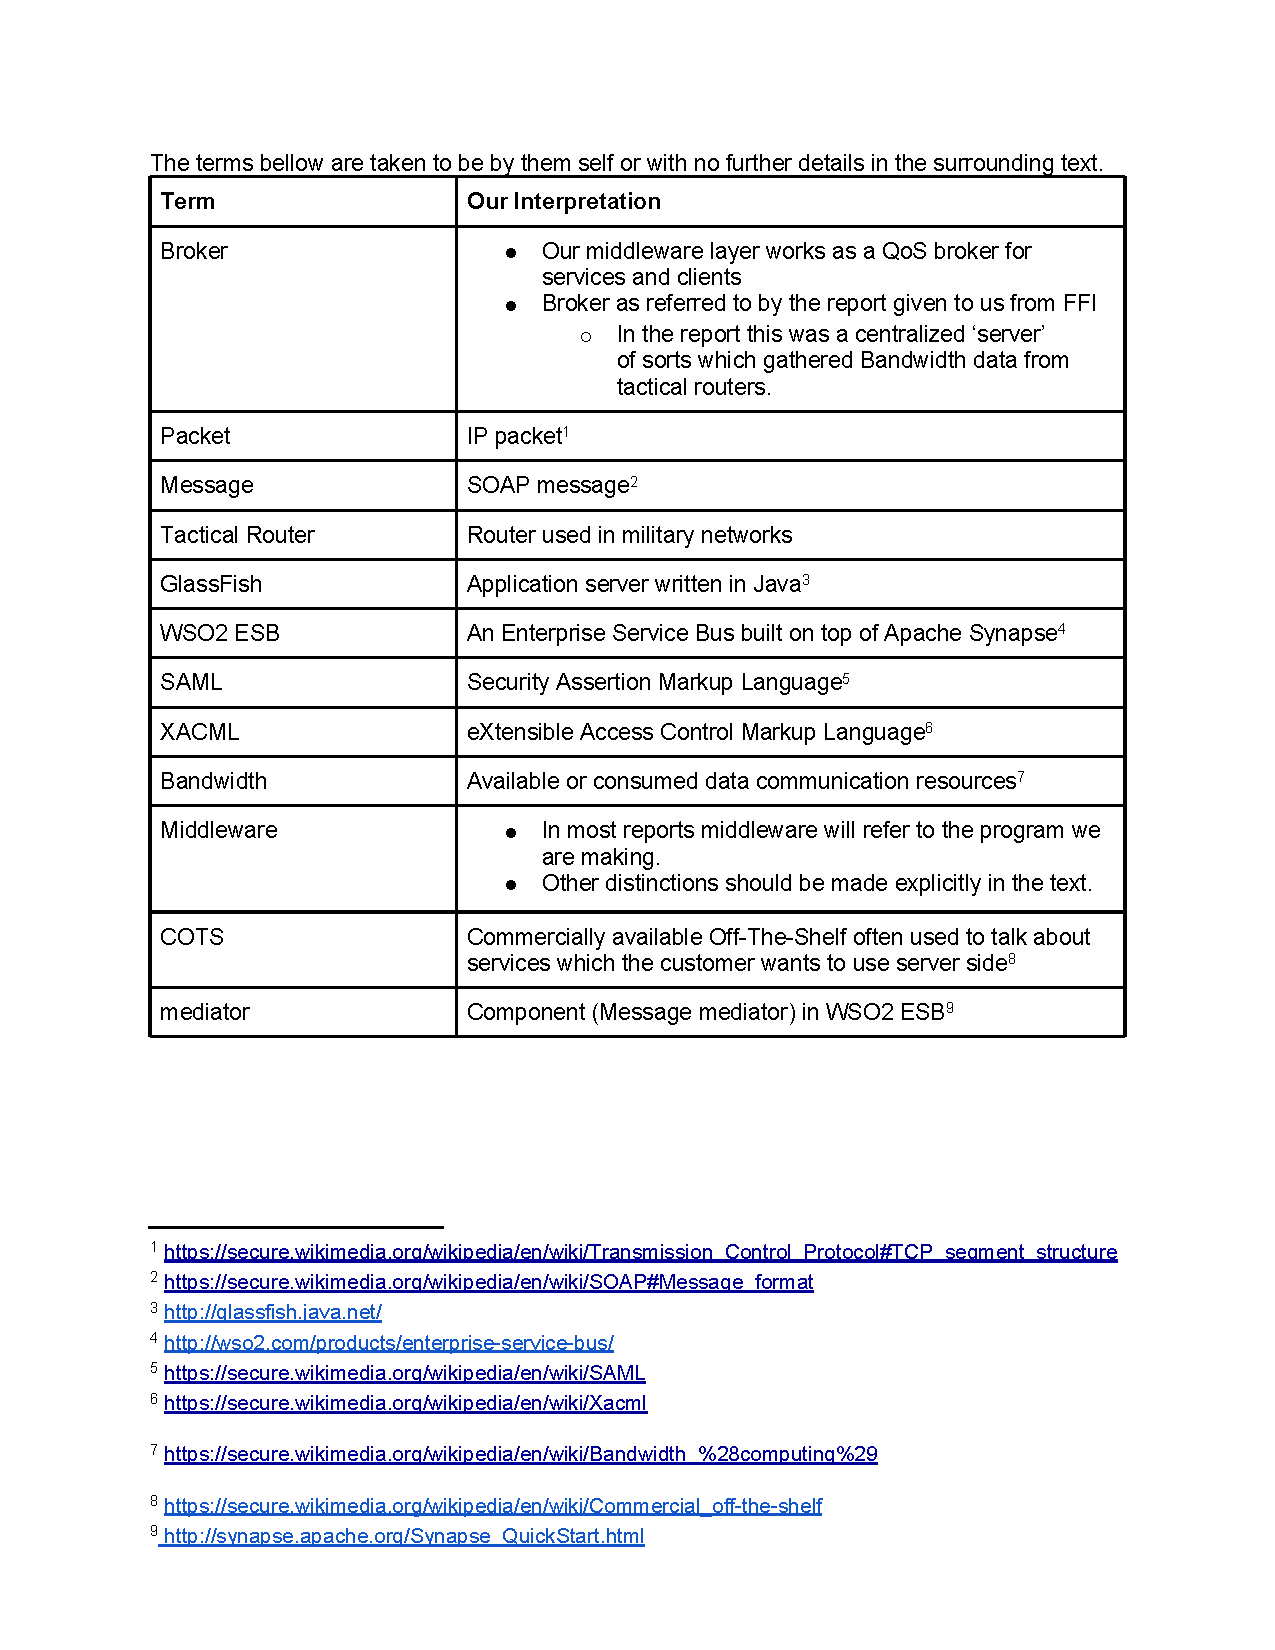
\includepdf{Glossary.pdf}
\section{File Attachments}\label{attachments}
    \attachfile[description=Risk List,icon=Paperclip]{risk.log} Risk List \\
    \attachfile[description=WBS,icon=Paperclip]{wbs.html} Work breakdown structure \\
    \\
    \attachfile[description=TEST log,icon=Paperclip]{report.log} Paperclip
    \attachfile[description=TEST log,icon=Graph]{report.log} Graph
    \attachfile[description=TEST log,icon=PushPin]{report.log} PushPin
    \attachfile[description=TEST log,icon=Tag]{report.log} Tag


\bibliographystyle{abbrv}
\bibliography{main}
\begin{thebibliography}{0}
    \bibitem{Dumy00} Dummy Dum,
        \emph{\LaTeX: A Dummy Bibliography Item}.
        Latex Experts, Lake Tahoe,
        4nd Edition,
        ca 1000.
\end{thebibliography}

\end{document}
